\documentclass[a4paper,10pt]{article}

  
  \usepackage[margin=1in,left=1.5in,includefoot]{geometry}
  \usepackage{graphics}

\begin{document}
  \begin{titlepage}
  \begin{center}
  \line(1,0){300}\\
  [.25in]
  \lhuge{\bfseries Operating System}\\
  [2mm]
  \line(1,0){200}\\
  [1.5cm]
  \textsc{\LARGE bangabandhu sheikh mujibur rahman science and technology university}\\
  [.75cm]
  \textsc{\small LaTex presentation}\\
  [10cm]
  \end{center}
 
  
  \begin{flushright}
  \textsc{\huge TARIKUL ISLAM}\\
  \Large 18ICTCSE011\\
  january,2020
  \end{flushright}
  \end{titlepage}
  
 %front matter stuff
 \pagenumbering{roman}
 \section*{Introduction}
 
  An Operating System (OS) is an interface between a computer user and computer hardware. An operating system is a software which performs all the basic tasks like file management, memory management, process management, handling input and output, and controlling peripheral devices such as disk drives and printers.

Some popular Operating Systems include Linux Operating System, Windows Operating System, VMS, OS/400, AIX, z/OS, etc. Coordination and assignment of compilers, interpreters, assemblers and other software to the various users of the computer systems.

An operating system is a program that acts as an interface between the user and the computer hardware and controls the execution of all kinds of programs.
\begin{figure}[h]
\centering
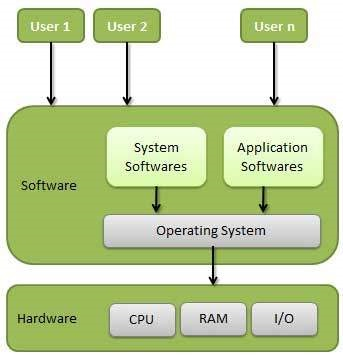
\includegraphics{addk}
\caption{Process}
\end{figure}
 \cleardoublepage
  
  %table of contents
  \tableofcontents
  \thispagestyle{empty}
  \cleardoublepage
  
  %main body stuff
  \pagenumbering{arabic}
  \setcounter{page}{1}  
  
  \section{Memory Management}
  Memory management refers to management of Primary Memory or Main Memory. Main memory is a large array of words or bytes where each word or byte has its own address.

Main memory provides a fast storage that can be accessed directly by the CPU. For a program to be executed, it must inthe main memory. An Operating System does the following activities for memory management$-$ 
 \begin{itemize}
  \item Keeps tracks of primary memory, i.e., what part of it are in use by whom, what part are not in use.
  \item In multiprogramming, the OS decides which process will get memory when and how much.
  \item Allocates the memory when a process requests it to do so
 
 \end{itemize}
 \begin{figure}[h]
 \centering
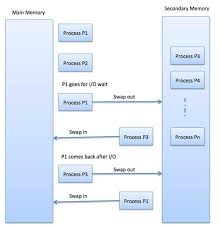
\includegraphics{mg}
\caption{Memory Management}
\end{figure}
 \section{Processor Management}
 In multiprogramming environment, the OS decides which process gets the processor when and for how much time. This function is called process scheduling. An Operating System does the following activities for processor management$-$
  \begin{itemize}
    \item Keeps tracks of processor and status of process. The program responsible for this task is known as traffic controller
    \item Allocates the processor (CPU) to a process.
    \item De-allocates processor when a process is no longer required.
  \end{itemize}
  \begin{figure}[h]
  \centering
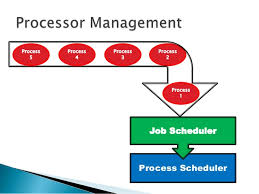
\includegraphics{pm}
\caption{Processor Management}
\end{figure}

  \newpage
  \section{Device Management}
An Operating System manages device communication via their respective drivers. It does the following activities for device management
 \begin{itemize}
   \item Keeps tracks of all devices. Program responsible for this task is known as the I/O controller$-$
   \item Decides which process gets the device when and for how much time.
   \item Allocates the device in the efficient way.

De-allocates devices.
 \end{itemize}
 \begin{figure}[h]
 \centering
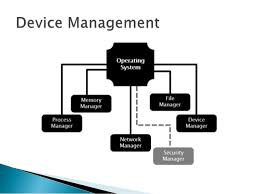
\includegraphics{dm}
\caption{Device Management}
\end{figure}
 
  \section{File Management}
A file system is normally organized into directories for easy navigation and usage. These directories may contain files and other directions.

An Operating System does the following activities for file management$-$
 \begin{itemize}
   \item Keeps track of information, location, uses, status etc. The collective facilities are often known as file system.
   \item Decides who gets the resources.

Allocates the resources.
   \item De-allocates the resources.
 \end{itemize}
 \begin{figure}[h]
 \centering
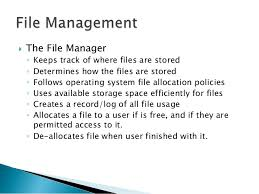
\includegraphics{fm}
\caption{File Management}
\end{figure}
   \newpage
  \section{Other Important Activities}
Following are some of the important activities that an Operating System performs$-$
  \begin{itemize}
    \item {\large Security} By means of password and similar other techniques, it prevents unauthorized access to programs and data.
    \item {\large Control over system performance} Recording delays between request for a service and response from the system.
    \item {\large Job accounting} Keeping track of time and resources used by various jobs and users. 
     \item {\large Error detecting aids}  Production of dumps, traces, error messages, and other debugging and error detecting aids.
     \item {\large Coordination between other softwares and users}  Coordination and assignment of compilers, interpreters, assemblers and other software to the various users of the computer systems.
  \end{itemize}
  
  \section{Batch operating system}
  The users of a batch operating system do not interact with the computer directly. Each user prepares his job on an off-line device like punch cards and submits it to the computer operator. To speed up processing, jobs with similar needs are batched together and run as a group. The programmers leave their programs with the operator and the operator then sorts the programs with similar requirements into batches.
  
The problems with Batch Systems are as follows$-$
  \begin{itemize}
    \item Lack of interaction between the user and the job.
    \item CPU is often idle, because the speed of the mechanical I/O devices is slower than the CPU.
    \item Difficult to provide the desired priority.
  \end{itemize}
  \begin{figure}[h]
  \centering
 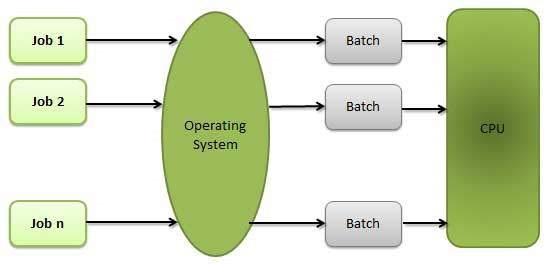
\includegraphics{batch}
\caption{Batch Processing}
\end{figure}
  \newpage
  
  \section{Difficult to provide the desired priority.}
  Time-sharing is a technique which enables many people, located at various terminals, to use a particular computer system at the same time. Time-sharing or multitasking is a logical extension of multiprogramming. Processor's time which is shared among multiple users simultaneously is termed as time-sharing.
  
The main difference between Multiprogrammed Batch Systems and Time-Sharing Systems is that in case of Multiprogrammed batch systems, the objective is to maximize processor use, whereas in Time-Sharing Systems, the objective is to minimize response time.

Multiple jobs are executed by the CPU by switching between them, but the switches occur so frequently. Thus, the user can receive an immediate response. For example, in a transaction processing, the processor executes each user program in a short burst or quantum of computation. That is, if n users are present, then each user can get a time quantum. When the user submits the command, the response time is in few seconds at most.

The operating system uses CPU scheduling and multiprogramming to provide each user with a small portion of a time. Computer systems that were designed primarily as batch systems have been modified to time-sharing systems$-$  


{\large Advantages of Timesharing operating systems are as follows}

 \begin{itemize}
   \item Provides the advantage of quick response.
   \item Avoids duplication of software.
   \item Avoids duplication of software.
 \end{itemize}
 
 {\large Disadvantages of Time-sharing operating systems are as follows}
   \begin{itemize}
     \item Problem of reliability.
     \item Question of security and integrity of user programs and data.
     \item Problem of data communication.
   \end{itemize}
   \newpage
 \section{Distributed operating System}
 Distributed systems use multiple central processors to serve multiple real-time applications and multiple users. Data processing jobs are distributed among the processors accordingly.
 
 The processors communicate with one another through various communication lines (such as high-speed buses or telephone lines). These are referred as loosely coupled systems or distributed systems. Processors in a distributed system may vary in size and function. These processors are referred as sites, nodes, computers, and so on.
 
The advantages of distributed systems are as follows$-$
  \begin{itemize}
     \item With resource sharing facility, a user at one site may be able to use the resources available at another.
     \item Speedup the exchange of data with one another via electronic mail.
     \item If one site fails in a distributed system, the remaining sites can potentially continue operating.
     \item Better service to the customers.
     \item Reduction of the load on the host computer.
     \item Reduction of delays in data processing.
  \end{itemize} 
  \newpage
  \section{Soft real-time systems}
  Soft real-time systems are less restrictive. A critical real-time task gets priority over other tasks and retains the priority until it completes. Soft real-time systems have limited utility than hard real-time systems. For example, multimedia, virtual reality, Advanced Scientific Projects like undersea exploration and planetary rovers, etc.
  
  An Operating System provides services to both the users and to the programs$-$
  \begin{itemize}
    \item Program execution
    \item I/O operations
    \item File System manipulation
    \item Communication
    \item Error Detection
    \item Resource Allocation
    \item Protection
 \end{itemize}  
 \subsection{Program execution}
 Operating systems handle many kinds of activities from user programs to system programs like printer spooler, name servers, file server, etc. Each of these activities is encapsulated as a process.

A process includes the complete execution context (code to execute, data to manipulate, registers, OS resources in use). Following are the major activities of an operating system with respect to program management$-$
 \begin{enumerate}
  \item Loads a program into memory.
   \item Executes the program.  
    \item Handles program's execution.
     \item Provides a mechanism for deadlock handling.
\end{enumerate}
\begin{figure}[h]
\centering
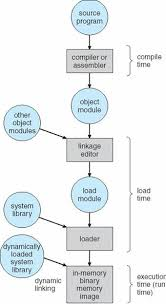
\includegraphics{pe}
\caption{Program Execution}
\end{figure} 
\newpage
 \subsection{I/O Operation}
  An I/O subsystem comprises of I/O devices and their corresponding driver software. Drivers hide the peculiarities of specific hardware devices from the users$-$
  \begin{enumerate}
   \item I/O operation means read or write operation with any file or any specific I/O device.
    \item Operating system provides the access to the required I/O device when required.
    
  \end{enumerate}
  \begin{figure}[h]
\centering
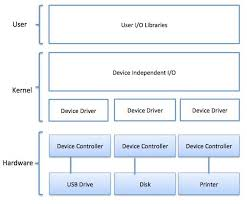
\includegraphics{io}
\caption{I/O Operation}
\end{figure} 
  
  
  \newpage
  \subsection{File system manipulation}
  A file represents a collection of related information. Computers can store files on the disk (secondary storage), for long-term storage purpose. Examples of storage media include magnetic tape, magnetic disk and optical disk drives like CD, DVD. Each of these media has its own properties like speed, capacity, data transfer rate and data access methods.

A file system is normally organized into directories for easy navigation and usage. These directories may contain files and other directions. Following are the major activities of an operating system with respect to file management$-$
 \begin{enumerate}
 \item Program needs to read a file or write a file.
  \item Permission varies from read-only, read-write, denied and so on.
Operating System provides an interface to the user to create/delete files.
   \item Operating System provides an interface to create the backup of file system.
 \end{enumerate}
  \subsection{Communication}
  In case of distributed systems which are a collection of processors that do not share memory, peripheral devices, or a clock, the operating system manages communications between all the processes. Multiple processes communicate with one another through communication lines in the network.

The OS handles routing and connection strategies, and the problems of contention and security. Following are the major activities of an operating system with respect to communication$-$
 \begin{enumerate}
  \item Two processes often require data to be transferred between them
   \item Both the processes can be on one computer or on different computers, but are connected through a computer network.
   \item Communication may be implemented by two methods, either by Shared Memory or by Message Passing.
 \end{enumerate}
 \newpage
  \subsection{Error handling}
  Errors can occur anytime and anywhere. An error may occur in CPU, in I/O devices or in the memory hardware. Following are the major activities of an operating system with respect to error handling$-$
  \begin{enumerate}
   \item The OS constantly checks for possible errors.
   \item The OS takes an appropriate action to ensure correct and consistent computing.
  \end{enumerate}
  \subsection{Resource Management}
  In case of multi-user or multi-tasking environment, resources such as main memory, CPU cycles and files storage are to be allocated to each user or job. Following are the major activities of an operating system with respect to resource management$-$
  \begin{enumerate}
   \item The OS manages all kinds of resources using schedulers.
   \item CPU scheduling algorithms are used for better utilization of CPU.
  \end{enumerate}
  \subsection{Protection}
  Considering a computer system having multiple users and concurrent execution of multiple processes, the various processes must be protected from each other's activities.

Protection refers to a mechanism or a way to control the access of programs, processes, or users to the resources defined by a computer system. Following are the major activities of an operating system with respect to protection$-$
 \begin{enumerate}
  \item The OS ensures that all access to system resources is controlled.
  \item The OS ensures that external I/O devices are protected from invalid access attempts.
  \item The OS provides authentication features for each user by means of passwords.
 \end{enumerate}
 \newpage
 
 \begin{figure}
 \centering
 
\includegraphics{op}
 
 \section{Networking}
 
 
Currently most operating systems support a variety of networking protocols, hardware, and applications for using them. This means that computers running dissimilar operating systems can participate in a common network for sharing resources such as computing, files, printers, and scanners using either wired or wireless connections. Networks can essentially allow a computer's operating system to access the resources of a remote computer to support the same functions as it could if those resources were connected directly to the local computer. This includes everything from simple communication, to using networked file systems or even sharing another computer's graphics or sound hardware. Some network services allow the resources of a computer to be accessed transparently, such as SSH which allows networked users direct access to a computer's command line interface.

Client/server networking allows a program on a computer, called a client, to connect via a network to another computer, called a server. Servers offer (or host) various services to other network computers and users. These services are usually provided through ports or numbered access points beyond the server's IP address. Each port number is usually associated with a maximum of one running program, which is responsible for handling requests to that port. A daemon, being a user program, can in turn access the local hardware resources of that computer by passing requests to the operating system kernel.

Many operating systems support one or more vendor-specific or open networking protocols as well, for example, SNA on IBM systems, DECnet on systems from Digital Equipment Corporation, and Microsoft-specific protocols (SMB) on Windows. Specific protocols for specific tasks may also be supported such as NFS for file access. Protocols like ESound, or esd can be easily extended over the network to provide sound from local applications, on a remote system's sound hardware.
 \end{figure}
\end{document}